\documentclass{sysuthesis}
%这是中山大学本科毕业论文非官方模版0.0.2的一部分
%维护者为陈颂光(1m02math@126.com)
%任何人可以自由使用本文件
%然而,无法保证它完全符合学校的相关要求,甚至不保证它可以正常编译
%对于使用此模版造成的任何后果,维护者不负有任何责任

%论文题目应以简短、明确的词语恰当概括整个论文的核心内容,避免使用不常见的缩略词、缩写字。读者通过标题可大致了解毕业设计(论文)的内容、专业的特点和科学的范畴。中文题目一般不宜超过 24 个字,必要时可增加副标题。外文题目一般不宜超过 12 个实词。
\title{中山大学本科毕业论文非官方模版}%论文题目
\author{陈颂光}%作者
\authorx{陈\ 颂\ 光}%封面上作者(各字符间可加空白)
\date{二〇一五年五月}%完成日期
\studentid{11336019}%学号
\school{数学与计算科学学院}%院(系)
\major{数学与应用数学}%专业
\mentor{老师姓名(职称)}%指导老师
%关键词是供检索用的主题词条(3—5 个),应采用能覆盖论文主要内容的通用技术词条(参照相应的技术术语标准)。按词条的外延层次排列(外延大的排在前面)。
\keywords{排版; 毕业论文; 模版}%中文关键词(每个关键词之间用“;”分开,最后一个关键词不打标点符号。)
\ekeywords{typeset; thesis; template}%英文关键词
\openingopinion{\rule{0cm}{6\baselineskip}}%开题报告中指导老师意见
\firstcheck{\rule{0cm}{6\baselineskip}}%第一次过程检查的学生总结
\firstopinion{\rule{0cm}{3\baselineskip}}%第一次过程检查的指导老师意见
\secondcheck{\rule{0cm}{6\baselineskip}}%第二次过程检查的学生总结
\secondopinion{\rule{0cm}{3\baselineskip}}%第二次过程检查的指导老师意见
\thirdcheck{\rule{0cm}{6\baselineskip}}%第三次过程检查的学生总结
\thirdopinion{\rule{0cm}{3\baselineskip}}%第三次过程检查的指导老师意见
\forthcheck{\rule{0cm}{6\baselineskip}}%第四次过程检查的学生总结
\forthopinion{\rule{0cm}{3\baselineskip}}%第四次过程检查的指导老师意见
\overallopinion{\rule{0cm}{8\baselineskip}}%整体完成情况的指导老师意见
\instructorcomment{\rule{0cm}{6\baselineskip}}%指导教师评语
\instructorgrade{\rule{0cm}{2\baselineskip}}%指导教师给予的成绩评定
\majorcomment{\rule{0cm}{4\baselineskip}}%答辩小组或专业负责人意见
\majorgrade{\rule{0cm}{2\baselineskip}}%答辩小组或专业负责人给予的成绩评定
\schoolcomment{\rule{0cm}{3\baselineskip}}%院系负责人意见
\schoolgrade{\rule{0cm}{2\baselineskip}}%院系负责人给予的成绩评定
\openingrep{
%接下来是开题报告内容
\paragraph{}开题报告内容	
}
\cabstract{
%摘要内容应概括地反映出本论文的主要内容,主要说明本论文的研究目的 、内容、方法、成果和结论。要突出本论文的创造性成果或新见解,不要与引言相混淆。语言力求精练、准确,以 300—500 字为宜。
%接下来是中文摘要内容
\paragraph{}中文摘要内容
}
\eabstract{
%英文摘要内容与中文摘要相同,以 250—400 个实词为宜。
%接下来是英文摘要内容
\paragraph{}Content of the abstract.
}
\begin{document}

\frontmatter

\cleardoublepage
\tableofcontents%目录
\cleardoublepage
\listoftables%表格目录(不需要则可以把这两行去掉)
\cleardoublepage
\listoffigures%插图目录(不需要则可以把这两行去掉)
\cleardoublepage
\listofalgorithms%算法目录(不需要则可以把这两行去掉)

\mainmatter


%现在开始正文

\chapter{引言}

\section{背景}

\paragraph{} 众所周知,编写毕业论文的过程如算法\ref{algor:write}所示。

\begin{algorithm}[H]
\KwData{字符串}
\KwResult{一篇毕业论文}
初始化\;
\While{当前时间未达到截止时间}{
	阅读现有内容\;
	\If{不知道自己在写什么}{
		重写\;
	}
}
\caption{编写毕业论文}
\label{algor:write}
\end{algorithm}

\section{国内外研究现状}

\paragraph{}国内外众多高校的毕业论文都有官方或非官方\LaTeX 模版,让莘莘学子从繁琐的排版细节中解放出来,得以集中精力于研究和写作工作本身。 

\section{本文工作}

\paragraph{}我们建立了一个尽可能符合《中山大学本科生毕业论文(设计)写作与印制规范》的\LaTeX 模版,容许任何人自由使用,然而我们无法保证它是否完全符合学校的相关要求,甚至不保证它可以正常编译\endnote{反正我是可以正常编译。}。对于使用此模版造成的任何后果,本人不负有任何责任。

\chapter{模版使用说明}

\section{正常使用}

\paragraph{}本模版主要组成部分有:

\begin{itemize}
\item {\ttfamily main.tex}为主文件,毕业论文的内容应放在这个文件中。
\item {\ttfamily main.bib}为参考文献记录。
\item {\ttfamily sysuthesis.bst}为参考文献样式文件。
\item {\ttfamily sysuthesis.cls}为文类文件,应与主文件放在相同的目录中。
\item {\ttfamily image/logo.png}为用在封面的校徽。
\end{itemize}

\paragraph{}主文件{\ttfamily main.tex}基本上是自解释的。在正常使用时,只用按照源文件中注释在正确位置填写各种基本信息、开题报告内容和中英文摘要内容,然后把注释``现在开始正文''到注释``篇末注''之间部分替换为正文,再按照注释在正确位置加入参考文献、致谢和附录等。最后用{\ttfamily xelatex}编译即可:

\begin{lstlisting}[language=bash, keywordstyle=\color{blue}\bfseries, basicstyle=\ttfamily, breaklines=true, frame=shadowbox]
xelatex main
bibtex main
xelatex main
xelatex main
\end{lstlisting}
。当然也可以用{\ttfamily makefile}或用脚本简化编译过程。

\section{配置}

\paragraph{}在使用本模版前,请先保证已安装以下宏包:

\begin{itemize}
\item {\ttfamily ctex}
\item {\ttfamily calc}
\item {\ttfamily graphicx}
\item {\ttfamily amsmath}
\item {\ttfamily amssymb}
\item {\ttfamily amsthm}
\item {\ttfamily listings}
\item {\ttfamily subfig}
\item {\ttfamily longtable}
\item {\ttfamily endnotes}
\item {\ttfamily algorithm2e}
\item {\ttfamily hyperref}
\end{itemize}

\paragraph{}为了让{\ttfamily algorithm2e}宏包支持中文,请把该宏包的文件{\ttfamily algorithm2e.sty}(在我的系统中,它在{\ttfamily /usr/share/texlive/texmf-dist/tex/latex/algorithm2e/})替换为本模版附带的同名文件。不需要描述算法时,可以在{\ttfamily sysuthesis.cls}中去掉以下代码
\begin{lstlisting}[language=TeX, keywordstyle=\color{blue}\bfseries, basicstyle=\ttfamily, breaklines=true, frame=shadowbox]
\RequirePackage[chinese,onelanguage,noline,noend,linesnumbered]{algorithm2e}
\end{lstlisting}
并在主文件中去掉以下代码
\begin{lstlisting}[language=TeX, keywordstyle=\color{blue}\bfseries, basicstyle=\ttfamily, breaklines=true, frame=shadowbox]
\listofalgorithms
\end{lstlisting}
(源文件有注释提示)。

\paragraph{}如果在windows编译且希望使用微软的字体时,请把{\ttfamily sysuthesis.cls}中以下代码
\begin{lstlisting}[language=TeX, keywordstyle=\color{blue}\bfseries, basicstyle=\ttfamily, breaklines=true, frame=shadowbox]
\LoadClass[adobefonts,a4paper,openright,cs4size,fancyhdr]{ctexbook}[2010/01/22]
\end{lstlisting}
改为
\begin{lstlisting}[language=TeX, keywordstyle=\color{blue}\bfseries, basicstyle=\ttfamily, breaklines=true, frame=shadowbox]
\LoadClass[winfonts,a4paper,openright,cs4size,fancyhdr]{ctexbook}[2010/01/22]
\end{lstlisting}。

\paragraph{}如果想使用开源字体{\ttfamily Fandol}(假定已安装它),请把{\ttfamily ctex}宏包的文件{\ttfamily ctex-xecjk-adobefonts.def}(在我的系统中,它在{\ttfamily /usr/share/ texlive/texmf-dist/tex/latex/ctex/fontset/})替换为本模版附带的同名文件。

\paragraph{}关于参考文献的bib条目格式参考\texttt{main.bib}~\cite{article}\cite{book}\cite{phdthesis}\cite{inproc}\cite{masterthesis}\cite{manual}\cite{report}\cite{database}\cite{software}\cite{standard}\cite{newspaper}\cite{patent}。

\chapter{写作时的注意事项}

\paragraph{}本章列出一些本模板未能规范也不太适合以注释形形式写在源文件的要求,请使用者注意。

\section{毕业论文的撰写内容与要求}

\paragraph{}正文一般包括以下几个方面:

\begin{enumerate}
\item 引言或背景\\
引言是论文正文的开端,应包括毕业论文选题的背景、目的和意义;对国内外研究现状和相关领域中已有的研究成果的简要评述;介绍本项研究工作研究设想、研究方法或实验设计、理论依据或实验基础;涉及范围和预期结果等。要求言简意赅,注意不要与摘要雷同或成为摘要的注解。
\item 主体\\
论文主体是毕业论文的主要部分,必须言之成理,论据可靠,严格遵循本学科国际通行的学术规范。在写作上要注意结构合理、层次分明、重点突出,章节标题、公式图表符号必须规范统一。论文主体的内容根据不同学科有不同的特点,一般应包括以下几个方面:
\begin{itemize}
\item 毕业论文(设计)总体方案或选题的论证;
\item 毕业论文(设计)各部分的设计实现,包括实验数据的获取、数据可行性及有效性的处理与分析、各部分的设计计算等;
\item 对研究内容及成果的客观阐述,包括理论依据、创新见解、创造性成果及其改进与实际应用价值等;
\item 论文主体的所有数据必须真实可靠,凡引用他人观点、方案、资料、数据等,无论曾否发表,无论是纸质或电子版,均应详加注释。自然科学论文应推理正确、结论清晰;人文和社会学科的论文应把握论点正确、论证充分、论据可靠,恰当运用系统分析和比较研究的方法进行模型或方案设计,注重实证研究和案例分析,根据分析结果提出建议和改进措施等。
\end{itemize}
\item 结论\\
结论是毕业论文的总结,是整篇论文的归宿,应精炼、准确、完整。结论应着重阐述自己的创造性成果及其在本研究领域中的意义、作用,还可进一步提出需要讨论的问题和建议。
\end{enumerate}

\section{毕业论文的撰写格式要求}

\paragraph{}除有特殊要求的专业外,毕业论文正文一般不少于 5000 字。各专业可根据需要确定具体的文字和字数要求,并报教务处备案。

\paragraph{}正文各部分的标题应简明扼要,不使用标点符号。

\paragraph{}名词术语的要求:

\begin{itemize}
\item 科学技术名词术语尽量采用全国自然科学名词审定委员会公布的规范词或国家标准、部标准中规定的名称,尚未统一规定或叫法有争议的名词术语,可采用惯用的名称。
\item 特定含义的名词术语或新名词、以及使用外文缩写代替某一名词术语时 , 首 次 出 现 时 应 在 括 号 内 注 明 其 含 义 , 如 : OECD ( Organisation for Economic Co-operation and Development) 代替经济合作发展组织。
\item 外国人名一般采用英文原名,可不译成中文,英文人名按姓前名后的原则书写,如:CRAY P,不可将外国人姓名中的名部分漏写,例如:不能只写CRAY, 应写成 CRAY P。一般很熟知的外国人名(如牛顿、爱因斯坦、达尔文、马克思等)可按通常标准译法写译名。
\end{itemize}

\paragraph{}物理量名称、符号与计量单位的要求:

\begin{itemize}
\item 论文中某一物理量的名称和符号应统一,一律采用国务院发布的《中华人民共和国法定计量单位》。单位名称和符号的书写方式,应采用国际通用符号。
\item 在不涉及具体数据表达时允许使用中文计量单位如“千克”。
\item 表 达 时 刻 应 采 用 中 文 计 量 单 位 , 如 “ 下 午 3 点 10 分 ” , 不 能 写 成“3h10min”,在表格中可以用“3:10PM”表示。
\item 物理量符号、物理量常量、变量符号用斜体,计量单位符号均用正体。
\end{itemize}

\paragraph{}数字的要求:

\begin{itemize}
\item 无特别约定情况下,一般均采用印度——阿拉伯数字表示。
\item 年份一律使用 4 位数字表示。
\item 小数的表示方法:一般情形下,小于 1 的数,需在小数点之前加 0。但当某些特殊数字不可能大于 1 时(如相关系数、比率、概率值),小数点之前的 0 要去掉,如 r=.26,p<.05。
\item 统计符号的格式:一般除 μ、α、β、λ、ε 以及 V 等符号外,其余统计符号一律以斜体字呈现,如ANCOVA , ANOVA , MANOVA , N , nl , M , SD , F , p , r 等。
\end{itemize}

\paragraph{}公式的要求:

\begin{itemize}
\item 公式应另起一行写在稿纸中央。一行写不完的长公式,最好在等号处转行,如做不到这一点,可在运算符号(如“+”、“-”号)处转行,等号或运算符号应在转行后的行首。
\item 公式的编号用圆括号括起,放在公式右边行末,在公式和编号之间不加虚线。公式可按全文统编序号,也可按章独立序号,如(49)或(4.11)。采用哪一种序号应和图序、表序编法一致。不应出现某章里的公式编序号,有的则不编序号。子公式可不编序号,需要引用时可加编 a、b、c......,重复引用的公式不得另编新序号。公式序号必须连续,不得重复或跳缺。
\item 文中引用某一公式时,写成“由式(16.20)”。
\end{itemize}

\paragraph{}表格的要求(表\ref{tab:skew}为一个也许不合格的例子):

\begin{itemize}
\item 表格必须与论文叙述有直接联系,不得出现与论文叙述脱节的表格。表格中的内容在技术上不得与正文矛盾。
\item 每个表格都应有自己的标题和序号。标题应写在表格上方正中,不加标点,序号写在标题左方。
\item 全文的表格可以统一编序,也可以逐章单独编序。采用哪一种方式应和插图、公式的编序方式统一。表序必须连续,不得跳缺。
\item 表格允许下页接写,接写时标题省略,表头应重复书写,并在右上方写“续表××”。多项大表可以分割成块,多页书写,接口处必须注明“接下页”、“接上页”、“接第×页”字样。
\item 表格应放在离正文首次出现处最近的地方,不应超前和过分拖后。
\end{itemize}

\begin{table}
\caption{各个倾斜校正方法性能对比}
\begin{tabular}{lrrrrr}
\hline
& 成功返回率 & 平均误差& 均方误差& 误差中位数& 运行时间中位数\\
& & (弧度) & (弧度) & (弧度) & (毫秒)\\\hline
参照方法&$\mathbf{100.00\%}$&0.1298&0.1504&0.1286&$\mathbf{0}$\\
分片填涂方法&93.48\%&0.0621&0.1947&0.0061&50\\
分片覆盖方法&99.10\%&0.0154&$\mathbf{0.0299}$&0.0073&300\\
投影方法&99.35\%&$\mathbf{0.0068}$&0.0335&$\mathbf{0.0033}$&197\\
交错数方法&99.35\%&0.0101&0.0458&0.0035&198\\
霍夫变换方法&99.35\%&0.1448&0.1827&0.0452&99\\
行间相关方法&93.81\%&0.2115&0.3811&0.0346&1615\\
最近邻方法&96.71\%&0.0883&0.1207&0.0690&67\\\hline
\end{tabular}
\label{tab:skew}
\end{table}

\paragraph{}图的要求(图\ref{fig:skew}为一个也许不合格的例子):

\begin{itemize}
\item 插图应与文字内容相符,技术内容正确。所有制图应符合国家标准和专业标准。对无规定符号的图形应采用该行业的常用画法。
\item 每幅插图应有标题和序号,全文的插图可以统一编序,也可以逐章单独编序,如:图 45 或图 6.8。采取哪一种方式应和表格、公式的编序方式统一。图序必须连续,不重复,不跳缺。
\item 由若干分图组成的插图,分图用 a、b、c......标序。分图的图名以及图中各种代号的意义,以图注形式写在图题下方,先写分图名,另起行写代号的意义。
\item 图与图标题、图序号为一个整体,不得拆开排版为两页。当页空白不够排版该图整体时,可将其后文字部分提前,将图移至次页最前面。
\item 对坐标轴必须进行文字标示,有数字标注的坐标图必须注明坐标单位。
\end{itemize}

\begin{figure}[htbp]
\centering
\subfloat[参照方法]{
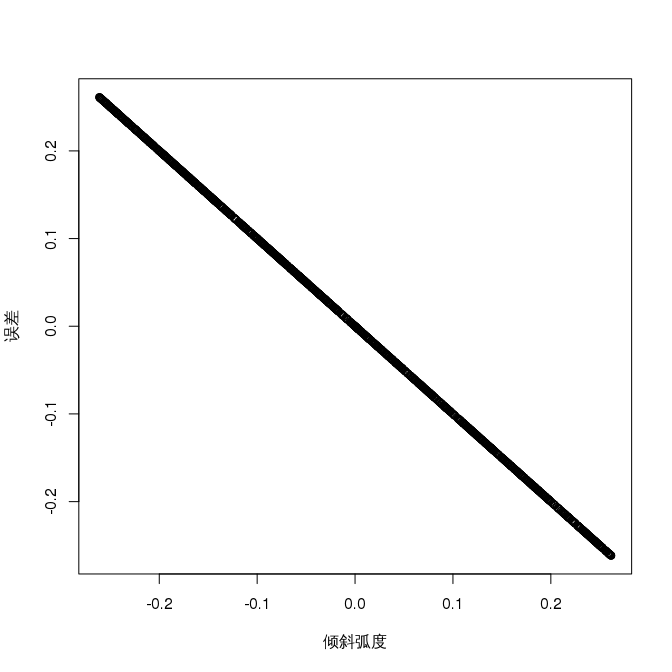
\includegraphics[scale=0.15]{image/err_ref.png}
}
\subfloat[分片填涂方法]{
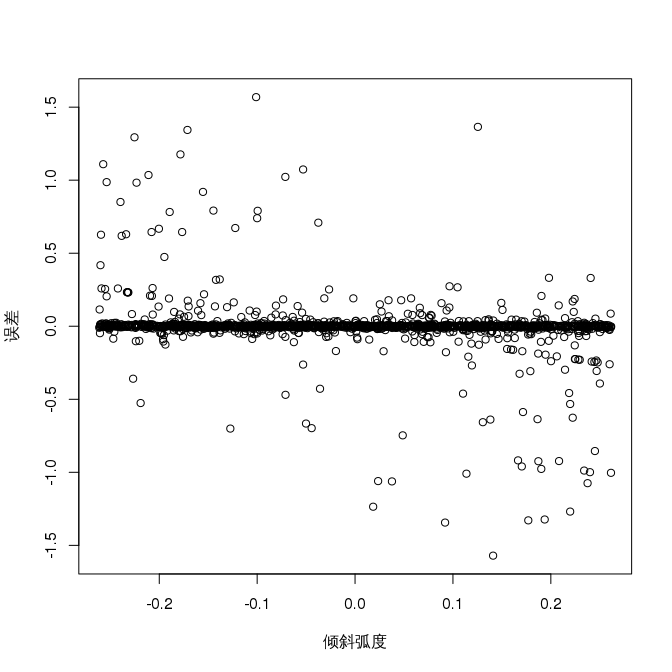
\includegraphics[scale=0.15]{image/err_ppa.png}
}\\
\subfloat[分片覆盖方法]{
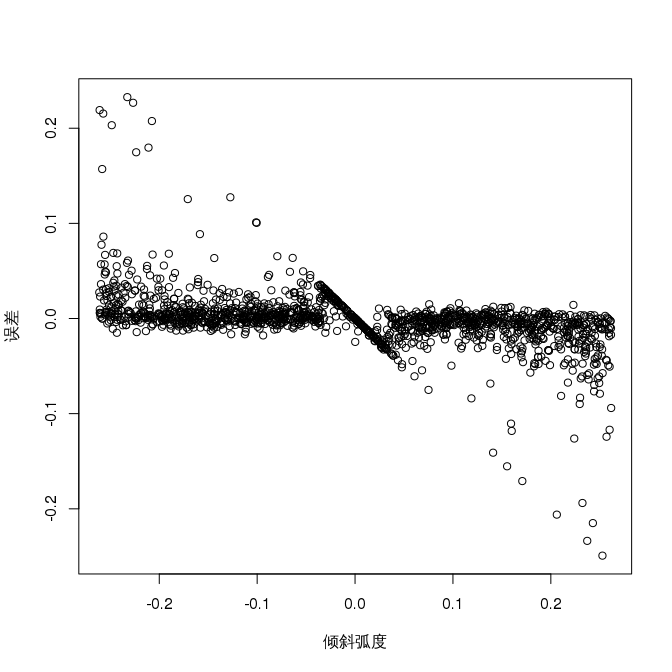
\includegraphics[scale=0.15]{image/err_pcp.png}
}
\subfloat[投影方法]{
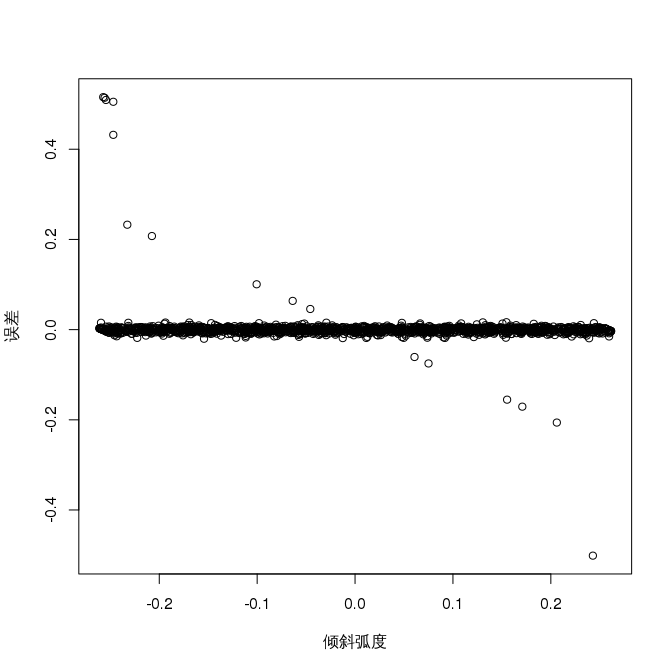
\includegraphics[scale=0.15]{image/err_pp.png}
}\\
\subfloat[交错数方法]{
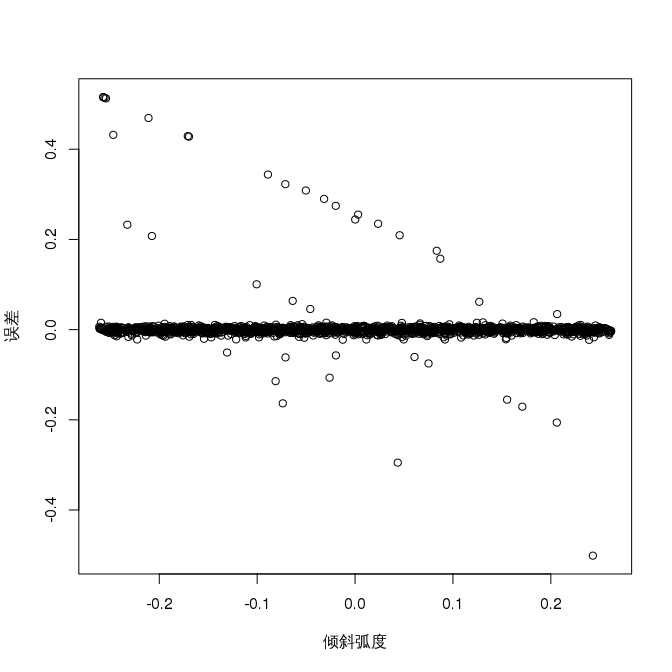
\includegraphics[scale=0.15]{image/err_tc.png}
}
\subfloat[霍夫变换方法]{
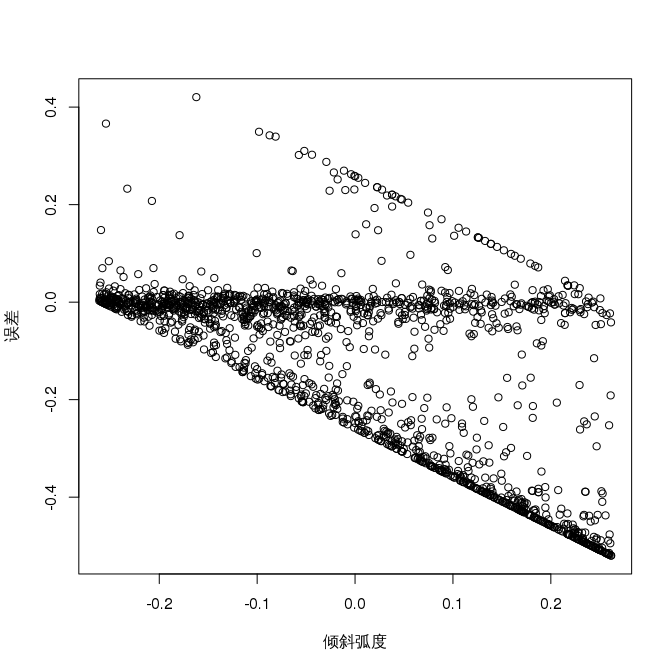
\includegraphics[scale=0.15]{image/err_ht.png}
}\\
\subfloat[行间相关方法]{
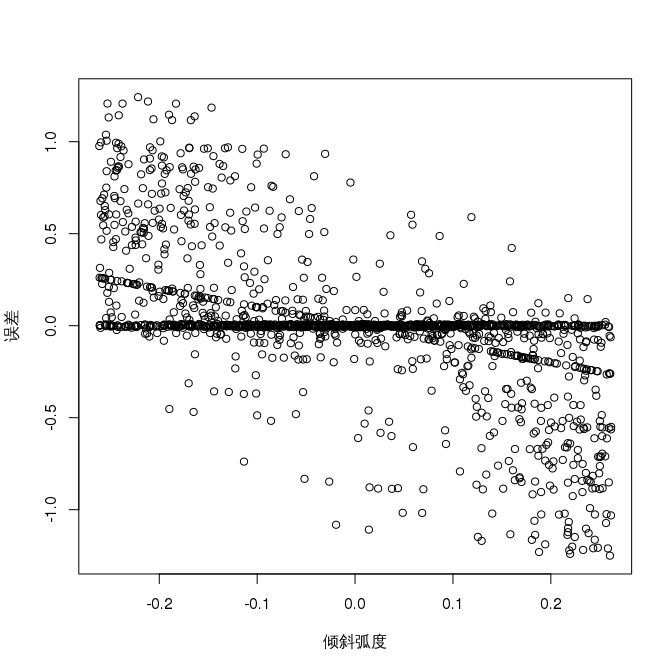
\includegraphics[scale=0.15]{image/err_cc.png}
}
\subfloat[最近邻方法]{
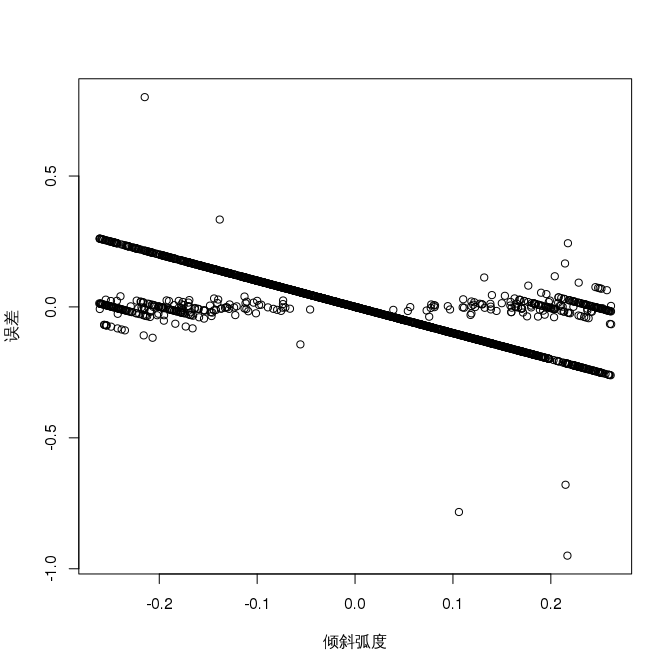
\includegraphics[scale=0.15]{image/err_nn.png}
}
\caption{各个倾斜校正方法的残差图}
\label{fig:skew}
\end{figure}

\chapter{结论}

\section{取得成果}

\paragraph{}一个大概不为人知的模版,可以认为对于人类无任何贡献。

\section{后续工作}

\paragraph{}此模版有以下已知局限性:

\begin{itemize}
\item 篇末注只支持最多10个
\item 有时用户可能要直接修改cls文件
\item 遗留了一些格式化代码在tex文件
\end{itemize}


%篇末注(非常抱歉只支持最多10个,在正文通过\endnote{}命令生成)
\displayendnotes

%参考文献是毕业设计(论文)不可缺少的组成部分,它反映毕业设计(论文)的取材来源、材料的广博程度和材料的可靠程度,也是作者对他人知识成果的承认和尊重。一份完整的参考文献可向读者提供一份有价值的信息资料,列入的文献应在 10 篇以上,其中外文文献在 2 篇以上。
\zihao{-5}\songti
\bibliographystyle{sysuthesis}
\bibliography{main}%假定bib文件为main.bib

\appendix

\chapter*{致谢}

\songti\zihao{-4}
%谢辞应以简短的文字对课题研究与论文撰写过程中曾直接给予帮助的人员(例如指导教师、答疑教师及其他人员)表示对自己的谢意,这不仅是一种礼貌,也是对他人劳动的尊重,是治学者应当遵循的学术规范。内容限一页。
%以下为致谢内容
\paragraph{}致谢内容

\vskip 18pt
\begin{flushright}
作者\\
\today
\end{flushright}

%对于一些不宜放在正文中的重要支撑材料,可编入毕业论文的附录中。包括某些重要的原始数据、详细数学推导、程序全文及其说明、复杂的图表、设计图纸等一系列需要补充提供的说明材料。如果毕业设计(论文)中引用的实例、数据资料,实验结果等符号较多时,为了节约篇幅,便于读者查阅,可以编写一个符号说明,注明符号代表的意义。附录的篇幅不宜太多,一般不超过正文。
%接下来是附录部分,以\chapter{附录标题}开始一个新的附录
\chapter{记号约定}
\songti\zihao{-4}
\begin{longtable}{ll}
记号 & 说明\\
\endfirsthead
记号 & 说明\\
\endhead
\endfoot
\endlastfoot
$A \cup B$ & 集合$A$与集合$B$的并集\\
$A \cap B$ & 集合$A$与集合$B$的交集\\
$A \setminus B$ & 集合$A$与集合$B$的差集\\
$A \times B$ & 集合$A$与集合$B$的直积\\
$A / \simeq$ & 集合$A$关于等价关系$\simeq$的商集\\
\end{longtable}

\backmatter

\end{document}
